%---------change this for every latex homework
\def\yourid{hz9xs}
\def\collabs{list collaborators's computing IDs}
\def\sources{Cormen, et al, Introduction to Algorithms.  \emph{(add others here)}}
% -----------------------------------------------------
\def\duedate{Friday, April 8, 2022 at 11:30 pm }
\def\duelocation{via Gradescope}
\def\htype{Adv}
\def\hunit{B}
\def\hnumber{}
\def\course{{cs4102 - algorithms - spring 2022}}%------
%-------------------------------------
%-------------------------------------

\documentclass[10pt]{article}
\usepackage[colorlinks,urlcolor=blue]{hyperref}
\usepackage[osf]{mathpazo}
\usepackage{amsmath,amsfonts,amssymb, graphicx}
\usepackage{latexsym}
\usepackage[top=1in,bottom=1.4in,left=1.25in,right=1.25in,centering,letterpaper]{geometry}
\usepackage{color}
\definecolor{mdb}{rgb}{0.1,0.6,0.4} 
\definecolor{cit}{rgb}{0.05,0.2,0.45} 
\pagestyle{myheadings}
\markboth{\yourid}{\yourid}
\usepackage{clrscode}
\usepackage{tabularx}
\newcolumntype{Y}{>{\centering\arraybackslash}X}

\newenvironment{proof}{\par\noindent{\it Proof.}\hspace*{1em}}{$\Box$\bigskip}
\newcommand{\handout}{
   \renewcommand{\thepage}{Unit \hunit: \htype~Homework \hnumber~-~\arabic{page}}
   \noindent
   \begin{center}
      \vbox{
    \hbox to \columnwidth {\sc{\course} \hfill}
    \vspace{-2mm}
       \hbox to \columnwidth {\sc due \MakeLowercase{\duedate} \duelocation\hfill {\Huge\color{mdb}\hunit\hnumber{\Large\MakeLowercase{\htype}}(\yourid)}}
      }
   \end{center}
   \vspace*{1mm}
   \hrule
   \vspace*{1mm}
    {\footnotesize \textbf{Collaboration Policy:} You are encouraged to collaborate with up to 3 other students, but all work submitted must be your own {\em independently} written solution. List the computing ids of all of your collaborators in the \texttt{collabs} command at the top of the tex file. Do not share written notes, documents (including Google docs, Overleaf docs, discussion notes, PDFs), or code.  Do not seek published or online solutions for any assignments. If you use any published or online resources (which may not include solutions) when completing this assignment, be sure to cite by naming the book etc.\ or listing a website's URL. Do not submit a solution that you are unable to explain orally to a member of the course staff. Any solutions that share similar text/code will be considered in breach of this policy. Please refer to the syllabus for a complete description of the collaboration policy.
   \vspace*{1mm}
    \hrule
    \vspace*{2mm}
    \noindent
    \textbf{Collaborators}: \collabs\\
    \textbf{Sources}: \sources}
    \vspace*{2mm}
    \hrule
    \vskip 2em
}

\newcommand{\solution}[1]{\color{blue}\hfill\break\noindent\textbf{Solution:} #1\color{black}}
%\newcommand{\altsolution}[1]{\color{blue}\hfill\break\noindent\textbf{Solution (Alternative):} #1\color{black}}

%\newcommand{\solution}[1]{}
\newcommand{\altsolution}[1]{}

\newcommand{\bit}[1]{\{0,1\}^{ #1 }}
%\dontprintsemicolon
%\linesnumbered
\newtheorem{problem}{\sc\color{cit}problem}
\newtheorem{practice}{\sc\color{cit}practice}
\newtheorem{lemma}{Lemma}
\newtheorem{definition}{Definition}
\newtheorem{theorem}{Theorem}

\newcommand{\Z}{\mathbb{Z}} % This might be useful for Integers!

\begin{document}
\thispagestyle{empty}
\handout

%----Begin your modifications here


%--------------------------------------------------------------------------
\begin{problem}Proof about MSTs\end{problem}

Let $e=(u,v)$ be a minimum-weight edge in an undirected connected graph $G$. Prove that $e=(u,v)$ belongs to some minimum spanning tree of G. 

\solution{
Prove by contradiction.
We assume $G'$ is a minimum spanning tree of $G$, and edge $e=(u,v)$ doesn't belong to $G'$. Let's add edge $e=(u,v)$ to $G'$ and there will be a cycle including edge $e$. In this cycle, let's remove another edge from $G'$. Notice that the new graph is also a spanning tree of $G$ and the weight of the edge we removed will be equal or greater than the weight of edge $e$ because edge $e$ has the minimum weight. So, after we remove an edge and add the edge $e=(u,v)$, the new graph's overall weight will be equal to or smaller than the weight of $G'$. If the new graph's overall weight is smaller than that of $G'$, $G'$ is not a minimum spanning tree, which is a contradiction, proving that $e$ belongs to a minimum spanning tree. If the new graph's overall weight is equal to the weight of $G'$, it shows that the new graph is also a minimum spanning tree and it contains $e$. So, for either case, $e=(u,v)$ must belongs to some minimum spanning tree of $G$.
}


%--------------------------------------------------------------------------
\begin{problem}\end{problem}

An airline, Gamma Airlines, is analyzing their network of airport connections.  They have a graph $G=(A,E)$ that represents the set of airports $A$ and their flight connections $E$ between them. They define $hops(a_i, a_k)$ to be the smallest number of flight connections between two airports.  They define $maxHops(a_i)$ to be the number of hops to the airport that is farthest from $a_i$, i.e. $maxHops(a_i) = max( hops(a_i, a_j) )\, \forall a_j \in A$.

The airline wishes to define one or more of their airports to be ``Core 1 airports.'' Each Core 1 airport $a_i$ will have a value of $maxHops(a_i)$ that is no larger than any other airport.  You can think of the Core 1 airports as being ``in the middle'' of Gamma Airlines' airport network.  The worst flight from a Core 1 airport (where ``worst'' means having a large number of connections) is the same or better than any other airport's worst flight connection (i.e.\ its $maxHops()$ value).

They also define ``Core 2 airports'' to be the set of airports that have a $maxHops()$ value that is just 1 more than that of the Core 1 airports.  (Why do they care about all this?  Delays at Core 1 or Core 2 airports may have big effects on the overall network performance.)

\textbf{Your problem: } Describe an algorithm that finds the set of Core 1 airports and the set of Core 2 airports.  Give its time-complexity.   The input is $G=(A,E)$, an undirected and unweighted graph, where $e = (a_i, a_j) \in E$ means that there is a flight between $a_i$ and $a_j$. Base your algorithm design on algorithms we have studied in this unit of the course.

\solution{
We do BFS to every vertices in the graph, and each BFS will generate a BFS tree for its corresponding starting node. Then, we compare the height of the tree for each BFS trees and get a set of smallest trees and second smallest trees(the height of second smallest tree equals to the height of smallest tree plus one). The corresponding starting node for those smallest trees are Core 1 airports. The corresponding starting node for those second smallest trees are Core 2 airports. Each BFS costs $\Theta (A+E)$, and we will do $A$ times so we have $\Theta(A*(A+E))$ time complexity. 
}



%--------------------------------------------------------------------------
\begin{problem}Vulnerable Network Nodes\end{problem}

Your security team has a model of nodes $v_i$ in your network where the relationship $d(v_i, v_j)$ defines if $v_j$ \emph{depends} on $v_i$. That is, if $d(v_i, v_j)$ is true,  the availability of second of these, $v_j$ relies on or depends on the availability of the first, $v_i$. We can represent this model of dependencies as a graph $G=(V,E)$ where $V$ is the set of network nodes and $e=(v_i, v_j) \in E$ means that $d(v_i, v_j)$ is true.  (For example, in the graph below, both H and J depend on F.)

Your team defines a \emph{vulnerable set} to be a subset $V'$ of the nodes in $V$ where all nodes in the subset depend on each other either directly or indirectly. (By ``indirectly'', we mean that $d(v_i, v_j)$ is not true, but $v_j$ depends on another node which eventually depends on $v_i$, perhaps through a ``chain'' of dependencies. For example, in the graph below, F depends on D indirectly.) 

\textbf{Your problem:}  Describe an algorithm (\textbf{and} give its time complexity) that finds the vulnerable set $VM$ in $G$ where 
\begin{enumerate}
\item the number of nodes in $VM$ is no smaller than the number of nodes in any other vulnerable set found in $G$, and
\item $\nexists \, v_i \in VM \textrm{ and } v_j \notin VM \textrm{ s.t. } d(v_i, v_j)$
\end{enumerate}
The second condition means that there are no nodes outside of VM that depend on any node in VM.

For example, in the graph below, there are a number of vulnerable sets, including $\{D, E, F\}, \{J, K\}$ and $\{G, H, I\}$.   The first of these does not meet the second condition. The other two do, but the last one is larger than the second one, so $VM=\{G, H, I\}$.

 
 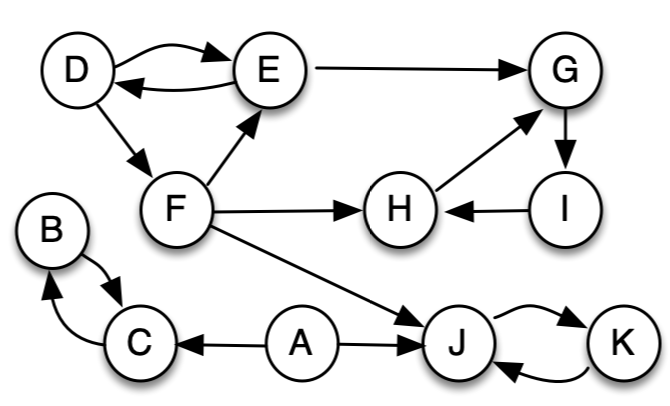
\includegraphics[width = 0.4\columnwidth]{vulnerable-sets.png}

\solution{
    \\
    1. Call DFS-sweep(G) to find finishing times u.f for each vertex u in G and to assign u.cc to each vertex. (Labeling Nodes in a Connected Components)\\
    2. Compute $G_T$, the transpose of digraph G. \\
    3. Call DFS-sweep($G_T$), do the recursive calls on nodes in the order
of decreasing u.f from Step 1. \\
    4. The DFS forest produced in Step 3 is the set of SCCs and we store the set with the number of nodes in each SCC. (and we need to pick the SCCs that meet condition 2 from this set of SCCs)\\
    5. Check every edges $e = (u, v)$ in $G$ to see if the nodes connected by the edge has the same cc value. If a pair of nodes have the same cc value, they are good. Otherwise, check dependency of node $u$ and $v$. If $u$ depends on $v$, SCCs containing $v$ does not meet condition 2 and thus we can remove these SCCs from the SCCs set in step 4. If $v$ depends on $u$, SCCs containing $u$ does not meet condition 2 and thus we can remove these SCCs from the SCCs set in step 4.\\
    6. For the rest of SCCs in the set, we need to compare the number of nodes they have. And the SCC with the highest number of nodes is the $VM$ we want to find.\\
    
    Time complexity: $\Theta(V+E)$.
}


\begin{problem} Gradescope Submission \end{problem}
Submit a version of this \verb|.tex| file to Gradescope with your solutions added, along with the compiled PDF.  You should only submit your \verb|.pdf| and \verb|.tex| files.


\end{document}

